\chapter{Marco Aplicativo}

\par En la investigación presentada se destaco la importancia de realizar pruebas de los sistemas de computo antes, durante y después de su desarrollo, los beneficios y dificultades que conlleva el despliegue de una nube híbrida, así como la relevancia de la inyección de fallas y la tendencia actual de este tipo de actividades de pruebas, debido a su importancia en los sistemas para mejorar el comportamiento de estos en caso de fallas.\\\\\\\\\\\\\\\\\\\\\\\\\\\\\\\\\\\\\\\\\\\\\\\\\\\\\\\\\\\\\\\\\\\\\\\\
\par Se planteo el desarrollo de un sistema automatizado con herramientas previamente definidas y comparadas, para obtener un entorno de pruebas e inyectar fallas a un clúster de Kubernetes, posteriormente con la respuesta obtenida podremos comparar el comportamiento del clúster al sufrir la falla con un estado óptimo previamente capturado, y establecer la respuesta del sistema a la falla tratada. Se utilizo Ansible para la automatización de las pruebas y así el usuario que utilice el sistema pueda escoger de manera controlada las fallas que desea inyectar. Con la ayuda de Minikube se desplegó un clúster de Kubernetes con un único nodo. Se despliega el clúster de Kurbenetes haciendo uso del container runtime Dockers para el despliegue de los Pods. El uso de estas herramientas sobre otras de similar propósito es respaldado por el hecho que son ampliamente utilizadas, son open source, existe el fácil acceso a la documentación y se posee conocimiento previo en el uso de estas.\\
%%%%%%%%%%%
\section{Objetivos}\label{sec:41}
\par Para el trabajo especial de grado se presentaron los siguientes objetivos:

%%%%%%%%%%%
\subsection{Objetivo General}


\par Estudiar la respuesta de un cluster de Kubernetes a fallas controladas en recursos de red, procesamiento y almacenamiento.

%%%%%%%%%%%
\subsection{Objetivos Específicos}
\begin{itemize}    
    \item Implementar un entorno básico que permita la ejecución de pruebas de inyección de fallas en un cluster de Kubernetes basadas en colecciones y roles de Ansible.
    \item Diseñar pruebas de inyección de fallas para causar interrupciones de servicio en un cluster de Kubernetes.
    \item Aplicar pruebas de inyección de fallas basadas en colecciones de Ansible para:
    \begin{itemize}
        \item Simular sobrecarga de CPU.
        \item Simular saturación de disco. 
        \item Introducir sobrecarga en las interfaces de red.
        \item Introducir latencia en la comunicación entre aplicaciones.
    \end{itemize}
    \item Caracterizar el comportamiento del cluster de Kubernetes en respuesta a la inyección de las fallas consideradas.
    \item Generar los resultados de las pruebas de inyección de fallas:
    \begin{itemize}
        \item Determinar si el sistema es capaz de recuperarse.
        \item Evaluar el posible tiempo de recuperación.
        \item Identificar, cuantificar y recolectar datos en caso de perdida de paquetes.
    \end{itemize}
\end{itemize}
%%%%%%%%%%%
\section{Metodología para el Desarrollo}


\par Las metodologías ágiles son ampliamente utilizadas en las operaciones de desarrollo por muchas organizaciones en la actualidad, su utilidad puede ser aplicada a la implementación de pruebas de inyección de fallas.\\ %\cite{LIB03}
\par En este se selecciono y aplico una metodología de desarrollo ágil, con las respectivas modificaciones que se mencionan posteriormente, con el fin de fomentar el proyecto. De las metodologías ágiles se selecciono Kanban, ya que ella fue la que mejor se adapto a los requerimientos de los experimentos de inyección de fallas a realizados. Su similar simplicidad con XP y uso en la actualidad en el desarrollo de software justifica el uso de Kanban, a su vez la carencia de tener que rellenar roles específicos y realizar eventos, lo ubica por encima sobre Scrum para su uso en el proyecto. La metodología Kanban, tiene principio y características  que justifican su utilización en el proyecto, entre los que destacan:
\begin{itemize}
    \item Flexibilidad en su aplicación: como marco de trabajo, Kanban es flexible y solo deben seguirse sus lineamientos y principios, en ningún caso limita las herramientas que se pueden utilizar, brindando notable independencia en el trabajo al equipo.
    \item Simplicidad: entre los mayores beneficios que tiene Kanban es su simplicidad, ya que contiene relativamente pocos roles a llenar y sólo requiere que se implementen unos pocos artefactos para almacenar la información necesaria y atender algunos eventos.
    \item Amplia flexibilidad a los cambios: Kanban acepta la posibilidad de modificaciones simples en su proceso y en las prioridades de desarrollo de éstos durante alguna iteración.
    \item Eficiencia: Kanban permite al equipo auto-organizarse y al integrar un diseño simple, permite incrementar la eficiencia del equipo de trabajo.
    \item Trabajo en equipo: el trabajo en equipo es aceptado en el método Kanban, que permite que exista una retroalimentación, mejorando la comunicación y optimizando el uso del tiempo.
\end{itemize} 
\par El marco de trabajo Kanban requirió de la siguiente modificación para adaptarse a las necesidades del proyecto:
\begin{itemize}
    \item Documentación y análisis de resultados: aunque muchos procesos ágiles como Kanban contemplan la documentación del trabajo mediante ciertos artefactos, ellos no inducen la recopilación de información de manera exhaustiva. Para poder adaptar este marco a nuestras necesidades de conveniente gestión del conocimiento, es necesario reunir y documentar toda la información posible en cada una de las etapas, analizar los resultados y compararlos con estados estables y/o anteriores. 
\end{itemize}
 
%%%%%%%%%%%
\section{Alcance}


\par En la actualidad, las organizaciones, sin importar su tamaño, requieren probar la fiabilidad de su entorno de cómputo híbrido en sus operaciones de desarrollo, para asegurar un servicio estable y confiable. Este proyecto propone estudiar la respuesta de un cluster de Kubernetes a fallas controladas en recursos de red, procesamiento y almacenamiento. El estudio está dirigido a aquellas organizaciones que deseen implementar experimentos de inyección de fallas en la nube híbrida, utilizando herramientas que pueden ser obtenidas con facilidad y a su vez probar la capacidad de sus servicios, en caso de eventos indeseables a lo largo de su desarrollo. \\

\par A su vez en el estudio se plantearan ciertas incógnitas sobre como se comporta Kubernetes ante ciertas fallas y se buscara responderlas.

%%%%%%%%%%%
\section{Arquitectura Propuesta}

\par El usuario ejecutara módulos de Ansible, lo cual
desencadenara la ejecución de un código de python en el nodo maestro de Kubernetes y así se inyectaran las fallas, apoyándonos con la API server de Kubernetes para acceder a todo el clúster. En la figura \ref{fig:arq02} se presenta la arquitectura básica propuesta.
\begin{figure}[htpb!]
	\centering
	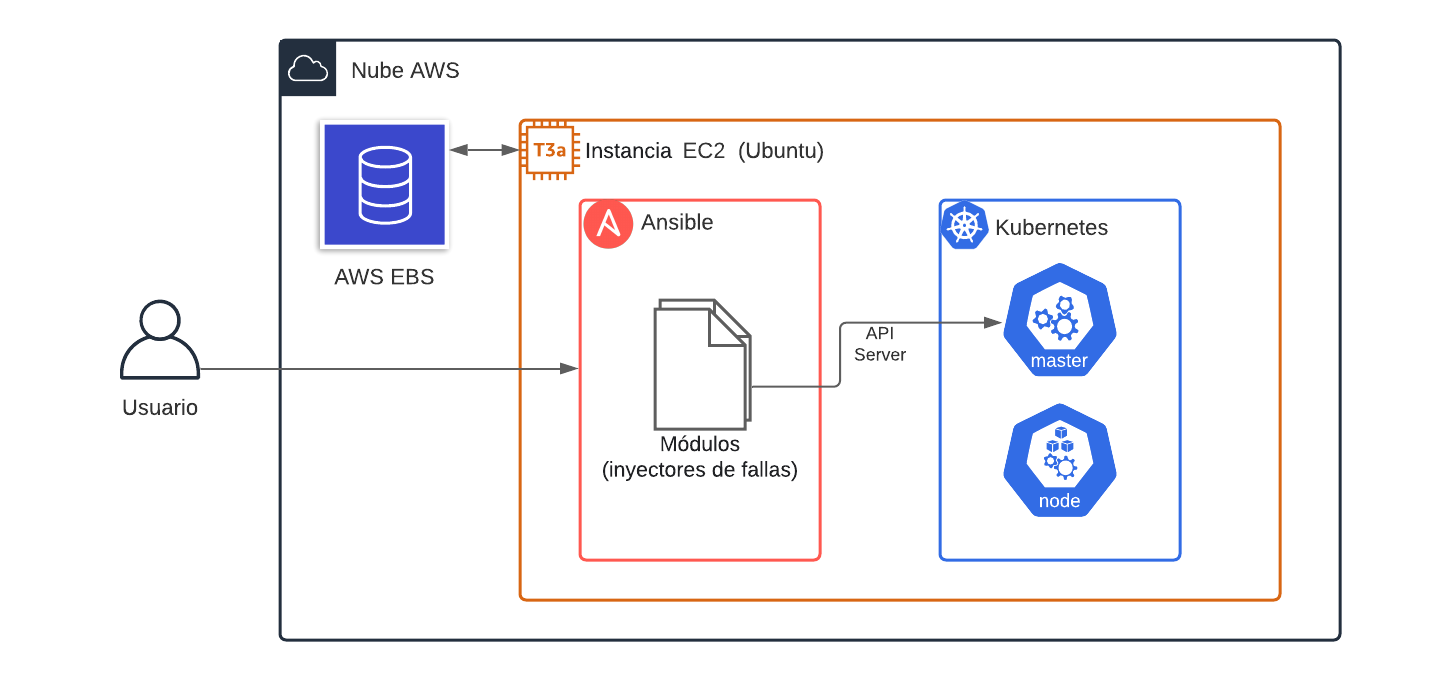
\includegraphics[width=0.95\columnwidth]{images/arq02.png}
	\caption{Arquitectura de la propuesta para el trabajo de grado.}
	\label{fig:arq02}
\end{figure}

\par Para la implementación anterior se plantea el uso de maquinas virtuales (VM), creando %2 instancias
una (1) instancia EC2 de AWS (Amazon Web Services) debido a que se posee conocimientos sobre este servicio y es de fácil acceso. La m\'aquina se configura con las siguientes características:

\begin{itemize}
    \item Para la instalación de Kubernetes de un solo nodo (Minikube) se configura una EC2 t3a.medium de AWS, con 2 vCPUs AMD EPYC 7000 de 2.5 GHz, 4GB de memoria RAM y sistema operativo Linux Ubuntu 20.04, a su vez se configura un AWS EBS de 8GB SSD para que funcione como la memoria en disco de dicha EC2.
\end{itemize}

\par A su vez fue necesaria la implementación de un ambiente local, en un equipo con capacidades de 32Gb de RAM, CPU de 4 núcleos y disco HDD. Fue configurada una maquina virtual para implementar un ambiente similar a la instancia de pruebas creada en AWS, la cual tiene las siguientes características:
\begin{itemize}
    \item La configuración cuenta también con la instalación de Kubernetes de un solo nodo (Minikube), la VM cuenta con dos 2 núcleos de CPU, a su vez cuenta con 4GB de memoria RAM, sistema operativo Linux Ubuntu 20.04 server, el adaptado de red fue configurado en modo puente (bridge) y cuenta con un almacenamiento de 20GB de disco virtual.
\end{itemize}
%%%%%%%%%%%

\section{Implementación}

\par Para la implementación del entorno y de los test de inyección de fallas, fue necesario realizar las actividades que se expondrán a continuación, que a su vez fueron divididas en subtareas, conforme a lo requerido al marco metodológico Kanban para poder diseñar y desarrollar dichos test. Algunas macro actividades derivan de los objetivos propuestos anteriormente en este capitulo y consistieron en:

\subsection{Implementación y despliegue del entorno de pruebas}

\par Para la implementación y despliegue del entorno de pruebas, propuesto en la arquitectura señalada anteriormente en este cap\'itulo, fue necesario el desarrollo de las tareas que se describen a continuación:\\

\subsubsection{Configuración de maquinas}
\par En lo que se refiere a la configuración de las maquinas necesarias para el desarrollo de este trabajo de investigación, se realizo la configuración de las maquinas expuestas con anterioridad en la sección 4.4 de este cap\'itulo, las cuales comparten características similares respecto a:
\begin{itemize}
    \item La instancia de AWS posee 2 vCPU y la instancia local tiene 2 núcleos de cpu, de 4 que posee el hardware.
    \item Ambas instancias poseen 4GB de memoria Ram configurada.
    \item Fue instalado el sistema operativo Linux Ubuntu 20.04 LTS para sevidores en ambas instancias (El sistema operativo fue seleccionado debido a que era una de las versiones mas actuales al momento de iniciar la investigación, siendo Ubuntu una de las distribuciones mas populares y usadas de Linux). 
\end{itemize}
\par Fue necesario el uso de un hypervisor (capa de software para realizar una virtualización de hardware) para configurar la m\'aquina virtual local. Se utilizo Vmware Workstation 15 Player como el hypervisor de preferencia, aunque otro hypervisor que permita el mismo nivel de configuración y personalizaci\'on de máquinas virtuales puede ser utilizado (como VirtualBox de Oracle), el Workstation 15 Player fue seleccionado solo porque  ya se posee conocimiento previo de esta herramienta.\\

\par Para disco, la m\'aquina local posee 20GB de disco virtual sobre un disco duro HDD, a diferencia de la instancia de AWS que solo se le configuro un EBS de 8GB de SSD.\\

\par En el ambiente local fue necesario la configuración del adaptador de red en modo Bridge para poder asignar a la maquina una dirección ip dentro de una red local para las pruebas, lo que permitió el fácil acceso al equipo a través de SSH, para la ejecución de comandos en esta maquina. El resumen de la configuración de la m\'aquina virtual local se puede observar en la imagen \ref{fig:vm01}, todos los demás aspectos de la configuración del hardware se aceptaron por defecto  de la herramienta de virtualizaci\'on.

\begin{figure}[htpb!]
	\centering
	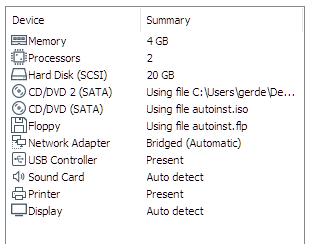
\includegraphics[width=0.70\columnwidth]{images/vm01.PNG}
	\caption{Arquitectura de la propuesta para el trabajo de grado.}
	\label{fig:vm01}
\end{figure}

\subsubsection{Instalación de herramientas: Minikube}

\par Las maquinas previamente mencionadas fueron configuradas con los requerimientos mínimos necesarios para la instalación de Minikube (Kubernetes de un solo nodo), también es necesario un container runtime como Docker (o similarmente compatible) o un entorno de máquina virtual. Para la instalación de Minikube se realizaron los siguientes pasos (todos los comandos son para el sistema operativo Linux Ubuntu 20.04 LTS server, para otros sistemas usar el comando de función similar):
\begin{enumerate}
    \item Se instala el container runtime (en este caso Docker), para este despliegue se realizo lo siguiente:
    \begin{itemize}
        \item Se actualiza la lista de paquetes existentes, usando el manejador de paquetes apt de Ubuntu:\begin{itemize}
            \item \textbf{sudo apt update}
        \end{itemize}
        \item Se instala algunos paquetes de requisitos previos que permitan a apt usar paquetes a través de HTTPS:
        \begin{itemize}
            \item \textbf{sudo apt install apt-transport-https ca-certificates curl software-properties-common}
        \end{itemize}
        \item Se añade la clave de GPG para el repositorio oficial de Docker en su sistema, tranferimos la llave desde curl que es una herramienta para tranferir data desde un servidor o a un servidor (con las banderas -fsSL, f para que en caso de falla no proporcione la salida, s para que no proporcione ningún mensaje del progreso, S solo despliegue un mensaje de error y L para seguir a la nueva ubicación en caso de que esta haya cambiado):
        \begin{itemize}
            \item \textbf{curl -fsSL https://download.docker.com/linux/ubuntu/gpg | sudo apt-key add -}
        \end{itemize}
        \item Se agrega el repositorio de Docker a las fuentes de apt:
        \begin{itemize}
            \item \textbf{sudo add-apt-repository ``deb [arch=amd64]\\ https://download.docker.com/linux/ubuntu focal stable''}
        \end{itemize}
        \item Se actualiza la lista de paquetes de nuevo con el repositorio de Docker agregado:
        \begin{itemize}
            \item \textbf{sudo apt update}
        \end{itemize}
        \item Se verifica que Docker se va a instalar desde el repositorio agregado con el comando:
        \begin{itemize}
            \item \textbf{apt-cache policy docker-ce}
        \end{itemize}
        \item Y se procede a instalar Docker con apt:
        \begin{itemize}
            \item \textbf{sudo apt install docker-ce}
        \end{itemize}
        \item Si se desea se puede verificar que Docker se instalo y esta en funcionamiento con:
        \begin{itemize}
            \item \textbf{sudo systemctl status docker}
        \end{itemize}
    \end{itemize}
    \item Antes de instalar Minikube, se instala el cliente de Kubernetes o kubectl a continuación:
    \begin{itemize}
        \item Se actualiza el repositorio apt:
        \begin{itemize}
            \item \textbf{sudo apt-get update}
        \end{itemize}
        \item Y se instalan los paquetes necesarios para usar el repositorio de Kubernetes en apt:
        \begin{itemize}
            \item \textbf{sudo apt-get install -y apt-transport-https ca-certificates curl}
        \end{itemize}
        \item Se descarga la llave de Google Cloud con curl:
        \begin{itemize}
            \item \textbf{sudo curl -fsSLo /usr/share/keyrings/kubernetes-archive-keyring.gpg \\https://packages.cloud.google.com/apt/doc/apt-key.gpg}
        \end{itemize}
        \item Luego se añade el repositorio de Kubernetes a apt:
        \begin{itemize}
            \item \textbf{echo ``deb[signed-by=/usr/share/keyrings/kubernetes-archive-keyring.gpg]\\ https://apt.kubernetes.io/ kubernetes-xenial main'' | sudo tee\\ /etc/apt/sources.list.d/kubernetes.list}
        \end{itemize}
        \item Se vuelve a actualizar apt:
        \begin{itemize}
            \item \textbf{sudo apt-get update}
        \end{itemize}
        \item Para instalar kubectl con apt:
        \begin{itemize}
            \item \textbf{sudo apt-get install -y kubectl}
        \end{itemize}
        \item Se verifica la instalación de kubectl:
        \begin{itemize}
            \item \textbf{kubectl version --client}
        \end{itemize}
    \end{itemize}
    \item Una vez instalado Docker y kubectl, se procede a realizar la instalacion de Minikube, el cual requiere que el equipo tenga por lo menos las siguientes características:
    \begin{itemize}
        \item 2 CPUs o mas.
        \item 2GB de memoria RAM o mas.
    \end{itemize}
    \item Luego se procede a obtener la descarga binaria de Minikube haciendo uso de curl (de nuevo con la bandera L para seguir a la ubicación y la bandera O para escribir el archivo remoto obtenido en un archivo local):
    \begin{itemize}
        \item \textbf{curl -LO https://storage.googleapis.com/minikube/releases/latest/minikube-linux-amd64}
    \end{itemize}
    \item Se instala Minikube con el siguiente comando: 
    \begin{itemize}
        \item \textbf{sudo install minikube-linux-amd64 /usr/local/bin/minikube}
    \end{itemize}
    \item Se inicia Minikube con los siguientes comandos:
    \begin{itemize}
        \item Si no se tiene acceso root: 
        %--driver=docker se usa en el primer inicio en caso de que se requiera especificar el driver de virtualizaci\'on, y se usa Docker debido a que es uno de los driver que pueden ser utilizados sin ser root
        \begin{itemize}
            \item \textbf{minikube start --drive=docker}
        \end{itemize}
        \item En caso de querer iniciar minikube con acceso root: 
        %en este comando no se especifica driver debido a que root no lo necesita y se asigna el apiserver a localhost
        \begin{itemize}
            \item \textbf{sudo minikube start --vm-driver=none --apiserver-ips 127.0.0.1 --apiserver-name localhost}
        \end{itemize}
    \end{itemize}
\end{enumerate}
\par Al culminar de realizar todos los pasos, se obtiene un instalación de Minikube con lo necesario para el depliegue de pods.


\subsubsection{Instalación de herramientas: Ansible}

\par Para la inyección de las fallas en el ambiente de Kubernetes de un solo nodo previamente instalado siguiendo los pasos anteriores, se propuso el uso de la herramienta de configuración  Ansible. Esta herramienta fue utilizada para la inyección de fallas y aplicar las pruebas basadas en colecciones de Ansible. Para poder instalar la herramienta se realizaron los siguientes pasos:
\begin{enumerate}
    \item Se inicia actualizando apt:
    \begin{itemize}
        \item \textbf{sudo apt update}
    \end{itemize}
    \item Se instala el archivo de paquetes personal o PPA, este software proporciona una abstracción de los repositorios de apt utilizados y permite administrar fácilmente la distribución y las fuentes de software de proveedores de software independientes:
    \begin{itemize}
        \item \textbf{sudo apt install software-properties-common}
    \end{itemize}
    \item Luego se agrega el repositorio de Ansible y actualiza el PPA:
    \begin{itemize}
        \item \textbf{sudo add-apt-repository --yes --update ppa:ansible/ansible}
    \end{itemize}
    \item Finalizar instalando Ansible con el comando:
    \begin{itemize}
        \item \textbf{sudo apt install ansible}
    \end{itemize}
\end{enumerate}

\par Después de ejecutar todos estos comandos, el ambiente deberia estar configura con todas las herramientas propuestas en la arquitectura.

\subsection{Diseño de test de inyección}
\par Al haber implementado el entorno de pruebas basado en tecnologías para el despliegue de entornos en la nube, se procedió a el diseño de las pruebas de inyección de fallas necesarias para poder caracterizar y poner a pruebas el ambiente desplegado. Se tomo en consideración para la elaboración de los test, las herramientas utilizadas como Minikube (Kubernetes de un solo nodo) y Ansible, por ello el uso de lenguajes como Python y de archivos de configuración YAML, debido a que estas herramientas proveen una buena integración  a través del uso de APIs y de un DSL. En el diseño de las pruebas se realizaron las siguientes actividades para poder cumplir con lo propuesto:

\subsubsection{Elaboración de Artefactos : Diagrama y especificación de Casos de Uso}
\par Para el desarrollo de los test de inyección de fallas basadas en colecciones y roles de Ansible, sobre un cluster de Kubernetes de un solo nodo se elaboraron los artefactos de casos de uso expuestos a continuación:\\


\textbf{Diagrama de Casos de Uso}\\


\par En la figura \ref{fig:uc01} se muestran los casos de uso identificados para el proyecto, con sus respectivas especificaciones:
% \begin{figure}[htpb!]
% 	\centering
% 	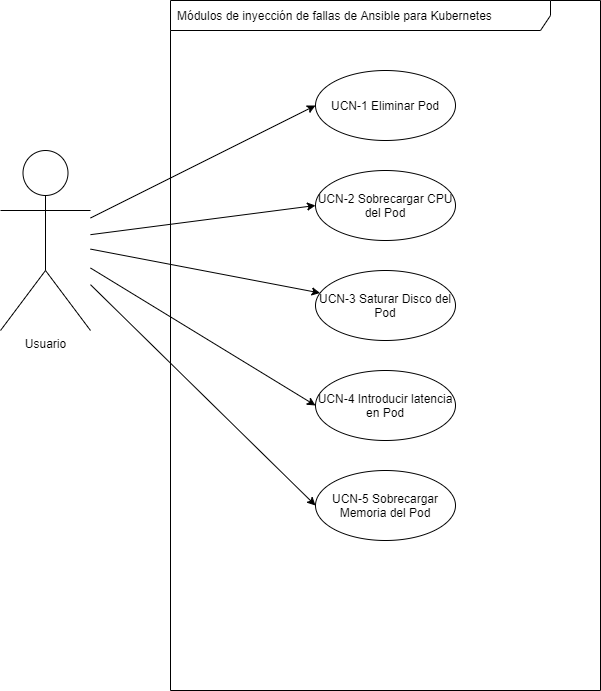
\includegraphics[width=0.70\columnwidth]{images/usecase/ucfaultinjectionfinal.png}
% 	\caption{Diagarama de Casos de Uso (UC) para los módulos de inyección de fallas en Ansible.}
% 	\label{fig:uc01}
% \end{figure}

\begin{figure}[htpb!]
	\centering
	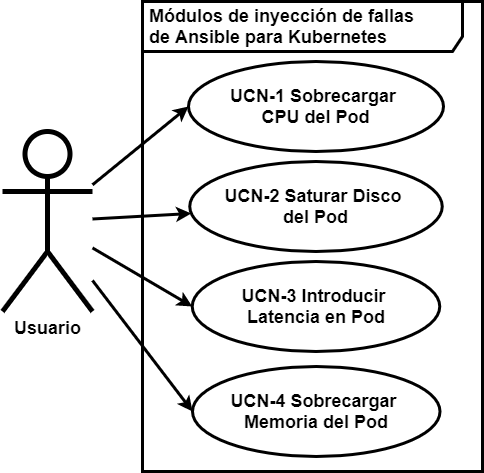
\includegraphics[width=0.795\columnwidth]{images/usecase/ucfaultinjectionF.png}
	\caption{Diagarama de Casos de Uso (UC) para los módulos de inyección de fallas en Ansible.}
	\label{fig:uc01}
\end{figure}

\textbf{Especificaciones de Casos de Uso}\\
% \par\textbf{UCN Eliminar Pod:}

% \begin{table}[htpb!]
% \tiny
% \centering
% \resizebox{\textwidth}{!}{%
% \begin{tabular}{|l|l|l|c|}
% \hline
% \rowcolor[HTML]{38FFF8}
% \textbf{UCN-1}   & \multicolumn{3}{l|}{\cellcolor[HTML]{38FFF8}\textbf{Eliminar Pod}} \\ \hline
% Dependencias     & \multicolumn{3}{l|}{Ninguna.} \\ \hline
% Precondición     & \multicolumn{3}{l|}{\begin{tabular}[c]{@{}l@{}}El usuario posee un ambiente de \\ kubernetes con un nodo de ansible \\ para ejecutar pruebas.\end{tabular}}  \\ \hline
% Descripción      & \multicolumn{3}{l|}{\begin{tabular}[c]{@{}l@{}}El módulo deberá comportarse \\ como se describe en el siguiente caso de uso \\ cuando el usuario desee eliminar uno o \\ varios Pods.\end{tabular}} \\ \hline
% Secuencia normal & Paso & \multicolumn{2}{l|}{Acción} \\ \hline & 1 & \multicolumn{2}{l|}{\begin{tabular}[c]{@{}l@{}}El usuario inicia la ejecución \\ del módulo a través de ansible \\ por consola.\end{tabular}} \\ \hline
%  & 2 & \multicolumn{2}{l|}{\begin{tabular}[c]{@{}l@{}}El usuario ejecuta el comando \\ para eliminar pods con los parámetros \\ necesarios como el namespace de pods a \\ eliminar, el nombre de un pod específico \\ a eliminar o si desea eliminar varios pods \\ aleatoriamente y la cantidad de estos.\end{tabular}} \\ \hline
%  & 3 & \multicolumn{2}{l|}{\begin{tabular}[c]{@{}l@{}}El modulo elimina el pod especifico o \\ la cantidad de pods requerida de manera \\ aleatoria, siguiendo una distribución \\ poisson por un periodo de tiempo que \\ define  $\lambda$ = 10.\end{tabular}} \\ \hline
%  & 4 & \multicolumn{2}{l|}{\begin{tabular}[c]{@{}l@{}}El sistema indica la finalización del módulo \\ sin error.\end{tabular}} \\ \hline
% Postcondición & \multicolumn{3}{l|}{\begin{tabular}[c]{@{}l@{}}El usuario observa cuales pods \\ fueron eliminados por el módulo.\end{tabular}} \\ \hline
% Excepciones & Paso & \multicolumn{2}{l|}{Acción} \\ \hline
%  & 2 & \multicolumn{2}{l|}{\begin{tabular}[c]{@{}l@{}}Si el usuario introduce algún parámetro \\ de forma errónea.\end{tabular}} \\ \hline
%   &  & E.1 & \begin{tabular}[c]{@{}l@{}}La ejecución del comando indica \\ en rojo por consola la falla del \\ parámetro erróneo.\end{tabular} \\ \hline

% \end{tabular}%
% }
% \end{table}

% \begin{table}[htpb!]
% \tiny
% \centering
% \resizebox{\textwidth}{!}{%
% \begin{tabular}{|l|l|l|c|}
% \hline
% \rowcolor[HTML]{38FFF8} 
% \textbf{UCN-1}   & \multicolumn{3}{l|}{\cellcolor[HTML]{38FFF8}\textbf{Eliminar Pod}} \\ \hline
%  &  & E.2 & El módulo finaliza su ejecución. \\ \hline
%  &  & E.3 & Se cancela el caso de uso. \\ \hline
% Comentarios & \multicolumn{3}{l|}{\begin{tabular}[c]{@{}l@{}}Los parámetros necesarios para la ejecución \\ son el nombre del namespace,  el nombre del \\ pod a eliminar o “random poisson” \\ (para eliminar aleatoriamente), la cantidad de \\ pods a eliminar (debe ser mayor o igual a 0 \\ para eliminación aleatoria e igual a 1 para un \\ pod específico) y la ubicación del intérprete \\ de python para ansible (la cual en Linux \\ por defecto es /usr/bin/python3).\end{tabular}} \\ \hline
% \end{tabular}%
% }
% \caption{Especificación de UCN1.}
% \label{tab:UCN1}
% \end{table}

\par\textbf{UCN-1 Sobrecargar CPU del Pod:}

\begin{table}[htpb!]
\tiny
\centering
\resizebox{\textwidth}{!}{%
\begin{tabular}{|l|l|l|l|}
\hline
\rowcolor[HTML]{38FFF8} 
\textbf{UCN-1} & \multicolumn{3}{l|}{\cellcolor[HTML]{38FFF8}\textbf{Sobrecargar CPU del Pod}} \\ \hline
Dependencias & \multicolumn{3}{l|}{Ninguna.} \\ \hline
Precondición & \multicolumn{3}{l|}{\begin{tabular}[c]{@{}l@{}}El usuario posee un ambiente de \\ kubernetes con un nodo de ansible \\ para ejecutar pruebas.\end{tabular}} \\ \hline
Descripción & \multicolumn{3}{l|}{\begin{tabular}[c]{@{}l@{}}El módulo deberá comportarse como \\ se describe en el siguiente caso de uso \\ cuando el usuario desee sobrecargar el CPU \\ de uno o varios Pods.\end{tabular}} \\ \hline
Secuencia normal & Paso & \multicolumn{2}{l|}{Acción} \\ \hline
 & 1 & \multicolumn{2}{l|}{\begin{tabular}[c]{@{}l@{}}El usuario inicia la ejecución del \\ módulo a través de ansible por consola.\end{tabular}} \\ \hline
 & 2 & \multicolumn{2}{l|}{\begin{tabular}[c]{@{}l@{}}El usuario ejecuta el comando para sobrecargar \\ el CPU de un pod con los parámetros necesarios \\ como el namespace del pod, el nombre de un pod \\ específico a sobrecargar o si desea sobrecargar varios\\  pods aleatoriamente, la cantidad de estos además de \\ la duración del experimento y la dirección\\ de red del ambiente de Kubernetes.\end{tabular}} \\ \hline
 & 3 & \multicolumn{2}{l|}{\begin{tabular}[c]{@{}l@{}}El módulo sobrecarga el CPU del pod \\ seleccionado o sobrecarga el cpu de la \\ cantidad de pods requerida de manera \\ aleatoria, siguiendo una distribución poisson \\ por un periodo de tiempo que define $\lambda$  = 10.\end{tabular}} \\ \hline
 & 4 & \multicolumn{2}{l|}{Se ejecuta el módulo de inyección de forma esperada.} \\ \hline
Postcondición & \multicolumn{3}{l|}{\begin{tabular}[c]{@{}l@{}}El usuario observa cuáles pods \\ fueron sometidos al módulo de \\ sobrecarga de CPU.\end{tabular}} \\ \hline
Excepciones & Paso & \multicolumn{2}{l|}{Acción} \\ \hline
 & 2 & \multicolumn{2}{l|}{\begin{tabular}[c]{@{}l@{}}Si el usuario introduce algún \\ parámetro de forma errónea.\end{tabular}} \\ \hline
 &  & E.1 & \begin{tabular}[c]{@{}l@{}}La ejecución del comando indica por \\ consola la falla del parámetro erróneo.\end{tabular} \\ \hline
 &  & E.2 & El modulo finaliza su ejecución. \\ \hline
 &  & E.3 & Se cancela el caso de uso. \\ \hline
 %& \multicolumn{3}{l|}{} \\
\end{tabular}%
}
\end{table}

\vspace{\baselineskip}
\vspace{\baselineskip}
\vspace{\baselineskip}

\begin{table}[htpb!]
\tiny
\centering
\resizebox{\textwidth}{!}{%
\begin{tabular}{|l|l|l|l|}
\hline
\rowcolor[HTML]{38FFF8} 
\textbf{UCN-1} & \multicolumn{3}{l|}{\cellcolor[HTML]{38FFF8}\textbf{Sobrecargar CPU del Pod}} \\ \hline
Comentarios & \multicolumn{3}{l|}{{\begin{tabular}[c]{@{}l@{}}Los parámetros necesarios para la \\ ejecución son el nombre del namespace, \\ el nombre del pod a sobrecargar  o “random poisson” \\ (para sobrecargar pods aleatoriamente), la cantidad de \\ pods a sobrecargar (debe ser mayor o igual a 0 para \\ sobrecarga aleatoria e igual a 1 para un pod específico), \\ la duración de ejecución del módulo (experimento) y \\ la ubicación del intérprete de python para ansible (la cual en \\ Linux por defecto es /usr/bin/python3).\end{tabular}}} \\ \hline
\end{tabular}%
}
\caption{Especificación de UCN-1.}
\label{tab:UCN1}
\end{table}

\vspace{\baselineskip}
\par\textbf{UCN-2 Saturar Disco del Pod:}

\begin{table}[htpb!]
\tiny
\centering
\resizebox{\textwidth}{!}{%
\begin{tabular}{|l|l|l|l|}
\hline
\rowcolor[HTML]{38FFF8} 
\textbf{UCN-2} & \multicolumn{3}{l|}{\cellcolor[HTML]{38FFF8}\textbf{Saturar Disco del Pod}} \\ \hline
Dependencias & \multicolumn{3}{l|}{Ninguna.} \\ \hline
Precondición & \multicolumn{3}{l|}{\begin{tabular}[c]{@{}l@{}}El usuario posee un ambiente de \\ kubernetes con un nodo de ansible \\ para ejecutar pruebas.\end{tabular}} \\ \hline
Descripción & \multicolumn{3}{l|}{\begin{tabular}[c]{@{}l@{}}El módulo deberá comportarse como se \\ describe en el siguiente caso de uso cuando \\ el usuario desee saturar el disco de uno o varios Pods.\end{tabular}} \\ \hline
Secuencia normal & Paso & \multicolumn{2}{l|}{Acción} \\ \hline
 & 1 & \multicolumn{2}{l|}{\begin{tabular}[c]{@{}l@{}}El usuario inicia la ejecución del módulo \\ a través de ansible por consola.\end{tabular}} \\ \hline
 & 2 & \multicolumn{2}{l|}{\begin{tabular}[c]{@{}l@{}}El usuario ejecuta el comando para saturar el disco \\ de un pod con los parámetros necesarios como el \\ namespace del pod, el nombre de un pod específico\\ a saturar el uso del disco o si desea saturar varios pods \\ aleatoriamente, la cantidad de estos, además de la \\ duración del experimento y la dirección\\ de red del ambiente de Kubernetes.\end{tabular}} \\ \hline
 & 3 & \multicolumn{2}{l|}{\begin{tabular}[c]{@{}l@{}}El modulo satura la memoria de disco del pod específico, \\ realizando operaciones de lectura/escritura durante el \\ periodo de tiempo.\end{tabular}} \\ \hline
 & 4 & \multicolumn{2}{l|}{Se ejecuta el módulo de inyección de forma esperada.} \\ \hline
Postcondición & \multicolumn{3}{l|}{\begin{tabular}[c]{@{}l@{}}El usuario observa el incremento en el uso \\ del disco de los pods ocasionado por el módulo \\ de saturar disco.\end{tabular}} \\ \hline
\end{tabular}%
}
\end{table}

\vspace{\baselineskip}
\vspace{\baselineskip}
\vspace{\baselineskip}

\begin{table}[htpb!]
\tiny
\centering
\resizebox{\textwidth}{!}{%
\begin{tabular}{|l|l|l|l|}
\hline
\rowcolor[HTML]{38FFF8} 
\textbf{UCN-2} & \multicolumn{3}{l|}{\cellcolor[HTML]{38FFF8}\textbf{Saturar Disco del Pod}} \\ \hline
Excepciones & Paso & \multicolumn{2}{l|}{Acción} \\ \hline
 & 2 & \multicolumn{2}{l|}{\begin{tabular}[c]{@{}l@{}}Si el usuario introduce algún parámetro de \\ forma errónea.\end{tabular}} \\ \hline
 &  & E.1 & \begin{tabular}[c]{@{}l@{}}La ejecución del comando indica por consola \\ la falla del parámetro erróneo.\end{tabular} \\ \hline
 &  & E.2 & El modulo finaliza su ejecución. \\ \hline
 &  & E.3 & Se cancela el caso de uso. \\ \hline
Comentarios & \multicolumn{3}{l|}{\begin{tabular}[c]{@{}l@{}}Los parámetros necesarios para la ejecución son \\ el nombre del namespace, el nombre del pod a ser \\ sometido a la saturación de disco  o “random poisson” \\ (para saturar pods aleatoriamente), la cantidad de pods a \\ saturar (debe ser mayor o igual a 0 para saturar aleatoriamente \\ e igual a 1 para un pod específico), la duración de ejecución \\ del módulo (experimento) y la ubicación del intérprete de python \\ para ansible (la cual en Linux por defecto es /usr/bin/python3).\end{tabular}} \\ \hline
\end{tabular}%
}
\caption{Especificación de UCN-2.}
\label{tab:UCN2}
\end{table}

\vspace{\baselineskip}
\par\textbf{UCN-3 Introducir latencia en Pod:}

\begin{table}[htpb!]
\tiny
\centering
\resizebox{\textwidth}{!}{%
\begin{tabular}{|l|l|l|l|}
\hline
\rowcolor[HTML]{38FFF8} 
\textbf{UCN-3} & \multicolumn{3}{l|}{\cellcolor[HTML]{38FFF8}\textbf{Introducir Latencia en Pod}} \\ \hline
Dependencias & \multicolumn{3}{l|}{Ninguna.} \\ \hline
Precondición & \multicolumn{3}{l|}{\begin{tabular}[c]{@{}l@{}}El usuario posee un ambiente de kubernetes \\ con un nodo de ansible para ejecutar pruebas.\end{tabular}} \\ \hline
Descripción & \multicolumn{3}{l|}{\begin{tabular}[c]{@{}l@{}}El módulo deberá comportarse como se \\ describe en el siguiente caso de uso cuando \\ el usuario desee introducir latencia en una \\ aplicación de uno o varios Pods.\end{tabular}} \\ \hline
Secuencia normal & Paso & \multicolumn{2}{l|}{Acción} \\ \hline
 & 1 & \multicolumn{2}{l|}{\begin{tabular}[c]{@{}l@{}}El usuario inicia la ejecución del módulo a través de ansible \\ por consola.\end{tabular}} \\ \hline
 & 2 & \multicolumn{2}{l|}{\begin{tabular}[c]{@{}l@{}}El usuario ejecuta el comando para introducir latencia \\ en la interfaz de red de un pod con los parámetros\\  necesarios como el namespace del pod, el nombre de \\ un pod específico a ser sometido al incremento de latencia, \\ que también es introducido por el usuario, o si desea afectar \\ varios pods aleatoriamente, la cantidad de estos, además de \\ la duración del experimento y la dirección\\ de red del ambiente de Kubernetes.\end{tabular}} \\ \hline
  & 3 & \multicolumn{2}{l|}{\begin{tabular}[c]{@{}l@{}}El módulo induce latencia en la interfaz \\ de comunicación de pods través de comandos.\end{tabular}} \\ \hline
 & 4 & \multicolumn{2}{l|}{\begin{tabular}[c]{@{}l@{}}Se ejecuta el módulo de inyección de \\ forma esperada.\end{tabular}} \\ \hline
\end{tabular}%
}
\end{table}

\begin{table}[htpb!]
\tiny
\centering
\resizebox{\textwidth}{!}{%
\begin{tabular}{|l|l|l|l|}
\hline
\rowcolor[HTML]{38FFF8} 
\textbf{UCN-3} & \multicolumn{3}{l|}{\cellcolor[HTML]{38FFF8}\textbf{Introducir Latencia en Pod}} \\
\hline
Postcondición & \multicolumn{3}{l|}{\begin{tabular}[c]{@{}l@{}}El usuario observa la respuesta de la aplicación \\ de los pods a otras aplicaciones que fue ocasionada\\  por el módulo que introduce latencia en la interfaz \\ de red de los pods.\end{tabular}} \\ \hline
Excepciones & Paso & \multicolumn{2}{l|}{Acción} \\ \hline
 & 2 & \multicolumn{2}{l|}{\begin{tabular}[c]{@{}l@{}}Si el usuario introduce algún parámetro de \\ forma errónea.\end{tabular}} \\ \hline
 &  & E.1 & \begin{tabular}[c]{@{}l@{}}La ejecución del comando indica por consola \\ la falla del parámetro erróneo.\end{tabular} \\ \hline
 &  & E.2 & El modulo finaliza su ejecución. \\ \hline
 &  & E.3 & Se cancela el caso de uso. \\ \hline
Comentarios & \multicolumn{3}{l|}{\begin{tabular}[c]{@{}l@{}}Los parámetros necesarios para la ejecución son el \\ nombre del namespace, el nombre del pod a ser sometido \\ al incremento de latencia  o “random poisson” (para afectar \\ pods aleatoriamente), la cantidad de pods a afectar (debe ser \\ mayor o igual a 0 para afectar aleatoriamente e igual a 1 para \\ un pod específico), la duración de ejecución del módulo (experimento),  \\ la ubicación del intérprete de python para ansible (la cual en Linux por \\ defecto es /usr/bin/python3) y la “cantidad” de latencia en milisegundos.\end{tabular}} \\ \hline
\end{tabular}%
}
\caption{Especificación de UCN-3.}
\label{tab:UCN3}
\end{table}

\vspace{\baselineskip}
\par\textbf{UCN-4 Sobrecargar Memoria del Pod:}

\begin{table}[htpb!]
\tiny
\centering
\resizebox{\textwidth}{!}{%
\begin{tabular}{|l|l|l|l|}
\hline
\rowcolor[HTML]{38FFF8} 
\textbf{UCN-4} & \multicolumn{3}{l|}{\cellcolor[HTML]{38FFF8}\textbf{Sobrecargar Memoria del Pod}} \\ \hline
Dependencias & \multicolumn{3}{l|}{Ninguna.} \\ \hline
Precondición & \multicolumn{3}{l|}{\begin{tabular}[c]{@{}l@{}}El usuario posee un ambiente de \\ kubernetes con un nodo de ansible \\ para ejecutar pruebas.\end{tabular}} \\ \hline
Descripción & \multicolumn{3}{l|}{\begin{tabular}[c]{@{}l@{}}El módulo deberá comportarse como se \\ describe en el siguiente caso de uso cuando \\ el usuario desee sobrecargar la memoria de uno \\ o varios Pods.\end{tabular}} \\ \hline
Secuencia normal & Paso & \multicolumn{2}{l|}{Acción} \\ \hline
 & 1 & \multicolumn{2}{l|}{\begin{tabular}[c]{@{}l@{}}El usuario inicia la ejecución del módulo a través \\ de ansible por consola.\end{tabular}} \\ \hline
 & 2 & \multicolumn{2}{l|}{\begin{tabular}[c]{@{}l@{}}El usuario ejecuta el comando para sobrecargar la \\ memoria de un pod con los parámetros necesarios como \\ el namespace del pod, el nombre de un pod específico a \\ sobrecargar o si desea sobrecargar varios pods aleatoriamente, \\  la cantidad de estos, además de la duración del experimento\\ y la dirección de red del ambiente de Kubernetes.\end{tabular}} \\ \hline
\end{tabular}%
}

\end{table}

\begin{table}[htpb!]
\tiny
\centering
\resizebox{\textwidth}{!}{%
\begin{tabular}{|l|l|l|l|}
\hline
\rowcolor[HTML]{38FFF8} 
\textbf{UCN-4} & \multicolumn{3}{l|}{\cellcolor[HTML]{38FFF8}\textbf{Sobrecargar Memoria del Pod}} \\ \hline
Secuencia normal & Paso & \multicolumn{2}{l|}{Acción} \\ \hline
 & 3 & \multicolumn{2}{l|}{\begin{tabular}[c]{@{}l@{}}El módulo sobrecarga la memoria del pod seleccionado \\ o sobrecarga la memoria de la cantidad de pods requerida \\ de manera aleatoria, siguiendo una distribución poisson por \\ un periodo de tiempo que define $\lambda$  = 10.\end{tabular}} \\ \hline
 & 4 & \multicolumn{2}{l|}{Se ejecuta el módulo de inyección de forma esperada.} \\ \hline
Postcondición & \multicolumn{3}{l|}{\begin{tabular}[c]{@{}l@{}}El usuario observa cuales pods fueron sometidos \\ al módulo de sobrecarga de memoria.\end{tabular}} \\ \hline
Excepciones & Paso & \multicolumn{2}{l|}{Acción} \\ \hline
 & 2 & \multicolumn{2}{l|}{Si el usuario introduce algún parámetro de forma errónea.} \\ \hline
 &  & E.1 & \begin{tabular}[c]{@{}l@{}}La ejecución del comando indica por consola la \\ falla del parámetro erróneo.\end{tabular} \\ \hline
 &  & E.2 & El modulo finaliza su ejecución. \\ \hline
 &  & E.3 & Se cancela el caso de uso. \\ \hline
Comentarios & \multicolumn{3}{l|}{\begin{tabular}[c]{@{}l@{}}Los parámetros necesarios para la ejecución son el nombre \\ del namespace, el nombre del pod a sobrecargar  o “random poisson” \\ (para sobrecargar pods aleatoriamente), la cantidad de pods a sobrecargar \\ (debe ser mayor o igual a 0 para sobrecarga aleatoria e igual a 1 para \\ un pod específico), la duración de ejecución del módulo (experimento) y \\ la ubicación del intérprete de python para ansible (la cual en Linux por \\ defecto es /usr/bin/python3).\end{tabular}} \\ \hline
\end{tabular}%
}
\caption{Especificación de UCN-4.}
\label{tab:UCN4}
\end{table}



\subsection{Desarrollo de test de inyección}
 %\subsubsection{Despliegue pystol}
 
 \carlos{Al inyectar los fallos debe haber una herramienta  que este generando las peticiones WEB, lectura/escritura, o inyectar trafico. Que herramienta estan utilizando, que parametros de configuracion tiene, por cuanto tiempo estan generando las peticiones?}
 
 \carlos{cuantos usuarios concurrentes estan lanzando las peticiones}
 
 \carlos{aqui tienen un ejemplo de el criterio para generar el trafico, https://k6.io/docs/test-types/stress-testing/}
 
 \carlos{piensen: que algoritmo tiene sentido que el cliente simule? Tiene sentido hacer un stress test, y aparte estamos lanzando Pystol? O buscamos simular el "comportamiento ideal"?}

\subsubsection{Desarrollo de funciones generales}
\par A continuación se explicaran las funciones de código que se reutilizan en cada test de inyección.

\begin{figure}[htpb!]
	\centering
	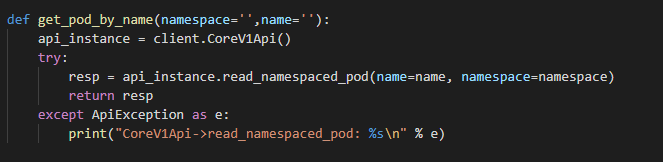
\includegraphics[width=0.90\columnwidth]{images/captures/codigo/Capture_get_pod_by_name.PNG}
	\caption{Captura del código de la función get\_pod\_by\_name().}
	\label{fig:codi01}
\end{figure}

\par En la figura \ref{fig:codi01} se muestra el código de la función  $\textbf{get\_pod\_by\_name(namespace, name)}$ la cual retorna la información de un pod a partir de su nombre, dicha función tiene como parámetros el namespace donde se encuentra el pod y su nombre. Ya que se utiliza la API del cliente de Kubernetes para Python se tiene acceso a la función \textbf{read\_namespaced\_pod(name, namespace)} la cual nos retorna el objeto con los detalles del pod. \\

\par Otra función importante de mencionar es \textbf{run\_module} la cual es básicamente el main de los tests de fallas, aquí se leen todos los parámetros recibidos por el modulo (nombre del pod a afectar, tiempo de la prueba, entre otros según el caso), se seleccionan los pod a afectar y es donde se llama a ejecutar la inyección de la falla.\\

\par También se hace gran uso de la herramienta \textbf{stress-ng} 
\carlos{que parametros se han utilizado?}
el cual fue diseñado para ejercitar varios subsistemas físicos de una computadora, así como las diversas interfaces del kernel del sistema operativo. La herramienta tiene una amplia gama de diferentes mecanismos de estrés (conocidos como "factores de estrés") de los cuales se hizo uso y se explicaran mas adelante.\\

\subsubsection{Desarrollo de test de inyección de latencia en interfaz de red}

\begin{figure}[htpb!]
	\centering
	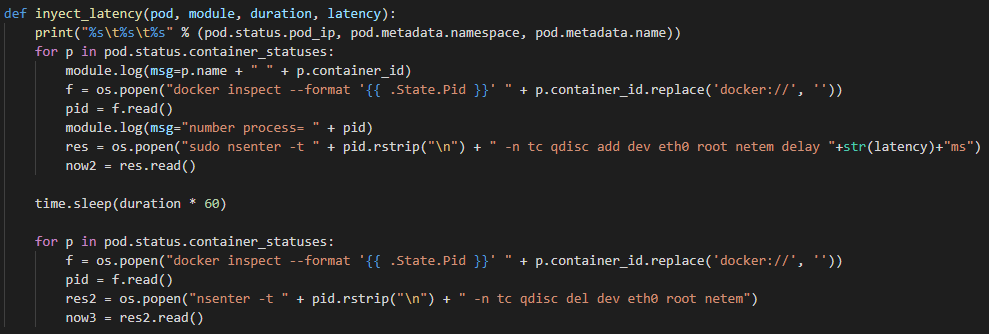
\includegraphics[width=0.95\columnwidth]{images/captures/codigo/Capture_inyect_latency.PNG}
	\caption{Captura del código de la función inyect\_latency().}
	\label{fig:codi02}
\end{figure}

\par En la figura \ref{fig:codi02} se puede observar la función \textbf{ inyect\_latency(pod, module, duration, latency)} la cual esta encargada de inyectar latencia en la interfaz de red de un pod.\\

\par La función recibe por parámetro los detalles del pod a probar, la instancia del modulo de ansible, la duración de la falla respectivamente y la cantidad en ms de latencia que el usuario quiera inyectar. \\

\par Utilizando el paquete os de Python se logra ejecutar comandos de linux en la maquina que corre el nodo y obtener las respuestas que estos devuelven. \\

\par En los detalles del pod se encuentra un atributo llamado container\_statuses el cual es una lista que tiene un tamaño equivalente al numero de contenedores que se ejecutan en el pod a afectar y en cada posición almacena la información del contenedor. Se realizaran ciclos sobre este arreglo para inyectar la latencia en cada contenedor y luego también para retirar dicho estrés.\\

\par Para inyectar la latencia en un contenedor primero se tiene que saber su ID de proceso, el cual se obtiene con el ejecutando el siguiente comando en el nodo \textbf{docker inspect --format '\{\{.State.Pid \}\}' <ID del contenedor>}, una vez tenemos el ID del proceso podemos ejecutar lo siguiente \textbf{sudo nsenter -t <ID del proceso> \ -n tc qdisc add dev eth0 root netem delay <latency>ms} a continuación una explicación por partes del comando:

\begin{itemize}
        \item nsenter -t <ID del proceso> \ -n: nsenter es una herramienta que permite ejecutar comandos en distintos namespaces de linux, con la bandera -t definimos el namespace objetivo pasándole como argumento el ID del proceso y el -n sin argumento lo que indica es que se utilice la red del proceso que se coloco como objetivo.
        \item tc: Herramienta utilizada para controlar el trafico de red en el kernel de Linux.
        \item qdisc add dev eth0 root: Con el comando qdisc podemos configurar la cola de almacenamiento de una interfaz de red, básicamente en esta sección del comando se esta agregando configuración (definida en el próximo punto) sin clase a la raíz del dispositivo eth0.
        \item netem delay <latency>ms: Esta es la configuración que es agregada a la interfaz, la que se menciono en el punto anterior, netem es un emulador de red que facilita agregar características a los paquetes que salen de una interfaz de red seleccionada, en este caso se agrega un retardo de N (latencia que pasa por parámetro el usuario) en milisegundos.\\
    \end{itemize}
    
\par Una vez todos los contenedores tenga agregada la latencia se esperan N segundos (duración de la falla la cual es agregada por el usuario vía parámetro en el modulo), por ultimo se elimina la configuración que agrega el retardo en la red de todos los contenedores.\\ 

\par Para ejecutar este modulo de inyección de fallas de latencia localmente, se configur\'o el siguiente comando:
\begin{itemize}
    \item \textbf{ansible -m include\_role \ -a `name=pystol.actions.networkstresspod' \ -e `$\{$ \\
    `pystol\_networkstresspod\_namespace': `<Namespace de los Pods>', \\
    `pystol\_networkstresspod\_pod': `<Nombre del Pod o aleatorio>', \\
    `pystol\_networkstresspod\_duration': `<Duracion de la Falla', \\
    `pystol\_networkstresspod\_amount': `<Cantidad de Pods>', \\
    `ansible\_python\_interpreter': `/usr/bin/python3', \\
    `pystol\_networkstresspod\_latency': `<Cantidad de Latencia en ms>'$\}$' \ localhost} %\ -vvvv}
\end{itemize}

\subsubsection{Desarrollo de test de inyección de sobrecarga de CPU}

\begin{figure}[htpb!]
	\centering
	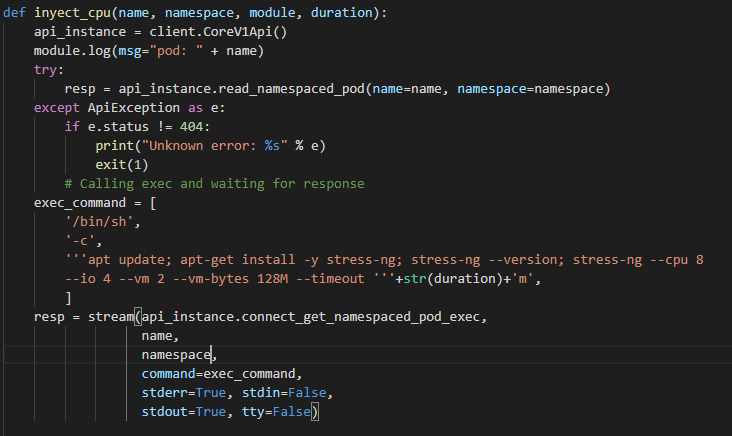
\includegraphics[width=0.95\columnwidth]{images/captures/codigo/Capture_inyect_cpu.PNG}
	\caption{Captura del código de la función inyect\_cpu().}
	\label{fig:codi03}
\end{figure}

\par En la figura \ref{fig:codi03} se puede observar la función \textbf{ inyect\_cpu(name, namespace, module, duration)} la cual esta encargada de inyectar la sobrecarga de CPU en un pod.\\
\par La función recibe por parámetro el nombre y el namespace del pod, la instancia del modulo de ansible y la duración de la falla respectivamente. \\
\par Inicialmente en esta función se crea una instancia de la API de Kubernetes para Python, luego se revisa si ciertamente existe un pod con el nombre y el namespace recibido por parámetros, a continuación se definen los comandos que se ejecutaran en el pod en los cuales se instala la herramienta stress-ng y se ejecuta la falla con el siguiente comando 
\textbf{stress-ng --cpu 8 --io 4 --vm 2 --vm-bytes 128M --timeout <duration>} a continuación una explicación de lo que significa cada bandera que se utiliza:
\carlos{esto no tiene mucho sentido, la prueba correcta sería, un pod con una aplicacion web, luego generan tráfico simulado con un criterio X, en ese momento lanzan la prueba desde ansible que satura el pod, miden como se comporta la aplicacion web, deja de responder? se crea otro pod?}
\begin{itemize}
        \item --cpu 8: Se inician 8 trabajadores que realizaran todos los trabajos de estress de CPU disponibles en stress-ng.
        \item --io 4: Se inician 4 trabajadores que realizan operaciones de entrada y salida en la cache del disco.
        \item --vm 2: Se inician 2 trabajadores que empiezan a hacer operaciones de escritura dentro de la memoria fisica asignada.        
        \item --vm-bytes 128M: Se le asignan 128 megabytes a cada trabajador de la bandera anterior.
        \item --timeout <duration>: Duración de la prueba.\\
    \end{itemize}

\par Por ultimo utilizando \textbf{stream} y \textbf{connect\_get\_namespaced\_pod\_exec} los cuales provienen de la API de Kubernetes, se logran ejecutar en el pod todos los comandos definidos previamente y recibir la respuesta.\\

\par Para ejecutar este modulo de inyección de fallas en CPU localmente, se configur\'o el siguiente comando:
\begin{itemize}
    \item \textbf{ansible -m include\_role \ -a `name=pystol.actions.cpustresspod' \ -e `$\{$ \\   
    `pystol\_cpustresspod\_namespace': `<Namespace de los Pods>',\\
    `pystol\_cpustresspod\_pod': `<Nombre del Pod o aleatorio>',\\
    `pystol\_cpustresspod\_duration': `<Duracion de la Falla>',\\
    `pystol\_cpustresspod\_amount': `<Cantidad de Pods>',\\
    `ansible\_python\_interpreter': `/usr/bin/python3'$\}$' \ localhost} % \ -vvvv}
\end{itemize}


\subsubsection{Desarrollo de test de inyección de sobrecarga de Memoria}

\begin{figure}[htpb!]
	\centering
	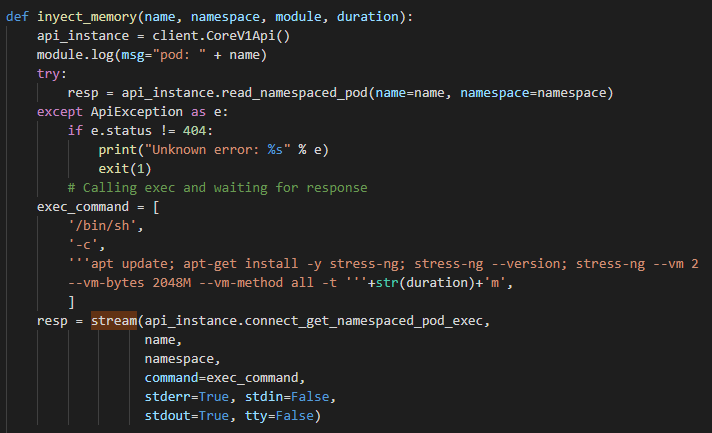
\includegraphics[width=0.95\columnwidth]{images/captures/codigo/Capture_inyect_memory.PNG}
	\caption{Captura del código de la función inyect\_memory().}
	\label{fig:codi04}
\end{figure}

\par En la figura \ref{fig:codi04} se puede observar la función \textbf{ inyect\_memory(name, namespace, module, duration)} la cual esta encargada de inyectar la sobrecarga en la memoria RAM de un pod.\\
\par La función recibe por parámetro el nombre y el namespace del pod, la instancia del modulo de ansible y la duración de la falla respectivamente. \\
\par Inicialmente en esta función se crea una instancia de la API de Kubernetes para Python, luego se revisa si ciertamente existe un pod con el nombre y el namespace recibido por parámetros, a continuación se definen los comandos que se ejecutaran en el pod en los cuales se instala la herramienta stress-ng y se ejecuta la falla con el siguiente comando
\textbf{stress-ng --vm 2 --vm-bytes 2048M --vm-method all -t <duration> } a continuación una explicación de lo que significa cada bandera que se utiliza:
\begin{itemize}
        \item --vm 2: Se inician 2 trabajadores que empiezan a hacer operaciones de escritura dentro de la memoria fisica asignada.        
        \item --vm-bytes 2048M: Se le asignan 2048 megabytes a cada trabajador de la bandera anterior.
        \item --vm-method all: Para que utilice todos los métodos disponibles en stress-ng de pruebas de memoria.
        \item -t <duration>: Duración de la prueba.\\
    \end{itemize}

\par Por ultimo utilizando \textbf{stream} y \textbf{connect\_get\_namespaced\_pod\_exec} los cuales provienen de la API de kubernetes, se logran ejecutar en el pod todos los comandos definidos previamente y recibir la respuesta.\\

\par Para ejecutar este modulo de inyección de fallas en memoria localmente, se configur\'o el siguiente comando:
\begin{itemize}
    \item \textbf{ansible -m include\_role \ -a `name=pystol.actions.memorystresspod' \ -e `$\{$ \\
    `pystol\_memorystresspod\_namespace': `<Namespace de los Pods>', \\
    `pystol\_memorystresspod\_pod': `<Nombre del Pod o aleatorio>', \\
    `pystol\_memorystresspod\_duration': `<Duracion de la Falla>', \\
    `pystol\_memorystresspod\_amount': `<Cantidad de Pods>', \\
    `ansible\_python\_interpreter': `/usr/bin/python3'$\}$' \ localhost} %\ -vvvv}
\end{itemize}



\subsubsection{Desarrollo de test de inyección de sobrecarga de Disco}

\begin{figure}[htpb!]
	\centering
	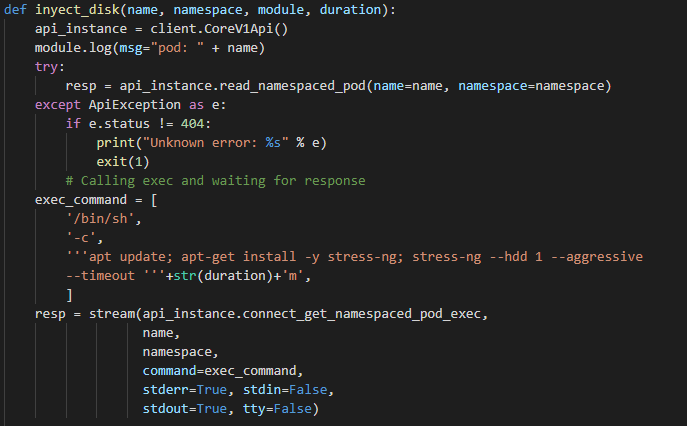
\includegraphics[width=0.95\columnwidth]{images/captures/codigo/Capture_inyect_disk.PNG}
	\caption{Captura del código de la función inyect\_disk().}
	\label{fig:codi05}
\end{figure}

\par En la figura \ref{fig:codi05} se puede observar la función \textbf{ inyect\_disk(name, namespace, module, duration)} la cual esta encargada de inyectar la sobrecarga en el disco.\\

\carlos{que es sobrecarga de disco?}

\par La función recibe por parámetro el nombre y el namespace del pod, la instancia del modulo de ansible y la duración de la falla respectivamente. \\
\par Inicialmente en esta función se crea una instancia de la API de Kubernetes para Python, luego se revisa si ciertamente existe un pod con el nombre y el namespace recibido por parámetros, a continuación se definen los comandos que se ejecutaran en el pod en los cuales se instala la herramienta stress-ng y se ejecuta la falla con el siguiente comando
\textbf{stress-ng --hdd 1 --aggressive --timeout <duration> } a continuación una explicación de lo que significa cada bandera que se utiliza:
\begin{itemize}
        \item --hdd 1: Se inicia un trabajador que escribe, lee y elimina archivos temporales en el disco.        
        \item --aggressive: Para que utilice todas las opciones disponibles en stress-ng que realicen operaciones de entrada y salida en el disco.
        \item --timeout <duration>: Duración de la prueba.\\
    \end{itemize}

\par Por ultimo utilizando \textbf{stream} y \textbf{connect\_get\_namespaced\_pod\_exec} los cuales provienen de la API de kubernetes, se logran ejecutar en el pod todos los comandos definidos previamente y recibir la respuesta.\\

\par Para ejecutar este modulo de inyección de fallas en disco localmente, se configur\'o el siguiente comando:
\begin{itemize}
    \item \textbf{ansible -m include\_role \ -a `name=pystol.actions.diskstresspod' \ -e `$\{$ \\
    `pystol\_diskstresspod\_namespace': `<Namespace de los Pods>', \\
    `pystol\_diskstresspod\_pod': `<Nombre del Pod o aleatorio>', \\
    `pystol\_diskstresspod\_duration': `<Duracion de la Falla>', \\
    `pystol\_diskstresspod\_amount': `<Cantidad de Pods>', \\
    `ansible\_python\_interpreter': `/usr/bin/python3'$\}$' \ localhost} %\ -vvvv}
\end{itemize}

\carlos{hace falta una tabla con los parametros de configuracion}

\subsection{Implementación y despliegue de herramientas para la experimentación}
\par Una vez teniendo las pruebas de inyección de fallas y el ambiente de estas implementado, fue necesario el despliegue de pods con características especificas para poder observar y caracterizar el comportamiento del cluster de Kubernetes con un solo nodo; también la obtención de métricas y resultados.\\
\subsubsection{Obtencion de metricas de Kubernetes: metrics-server}

\par Las métricas de uso de los recursos, como la CPU del pod y el uso de la memoria de este, están disponibles en Kubernetes a través de la API de métricas. Un usuario puede acceder a estas métricas directamente con un comando o un controlador en el clúster, por ejemplo el controlador encargado de escalar los pods horizontalmente. Metrics-Server es un agregador de datos de uso de recursos y es un componente a nivel de clúster que periódicamente extrae las métricas de todos los nodos de Kubernetes que ofrece Kubelet. A través de la API de métricas, puede obtener la cantidad de recursos que utiliza actualmente un nodo o un pod determinado, esta API no almacena los valores de las métricas, por lo que no es posible obtener valores de uso históricos sin el uso de herramientas de terceros \cite{WEB03}. Al consultar el servidor por linea de comandos se pueden obtener las siguientes métricas: 
\begin{itemize}
    \item \textbf{CPU:} El uso de CPU se informa como el uso promedio, en núcleos de CPU, durante un período de tiempo, este valor se obtiene tomando una tasa sobre un contador de CPU acumulativo proporcionado por el kernel (tanto en Linux como Windows) y Kubelet elige la ventana de tiempo para el cálculo del valor.
    \item \textbf{Memoria:} La memoria se informa como el \textit{working set} o ``conjunto de trabajo'', en bytes, en el instante en que se recopiló la métrica, el \textit{working set} es la cantidad de memoria en uso que no se puede liberar bajo la presión de la memoria. Sin embargo, el cálculo del conjunto de trabajo varía según el sistema operativo del host y por lo general, se produce una estimación. Incluye toda la memoria anónima (no respaldada en archivos), ya que Kubernetes no admite el swap, la métrica también incluye algo de memoria en caché (respaldada por archivos), porque el sistema operativo del host no siempre puede reclamar dichas páginas.
\end{itemize}

\par Para hacer uso del metrics-server por comandos es necesario realizar los pasos a continuación:
\begin{enumerate}
    \item Se ejecuta el siguiente comando para habilitar el servidor de metricas dentro del cluster (es necesario levantar Minikube):
    \begin{itemize}
        \item \textbf{minikube addons enable metrics-server}
    \end{itemize}
    \item Una vez habilitado metrics-server se puede consultar la ultima medicion realizada con:
    \begin{itemize}
        \item \textbf{kubectl top}
        \item \textbf{kubectl top pods} para obtener los recursos utilizados por los pods.
    \end{itemize}
\end{enumerate}

\subsubsection{Implementación y despliegue de pods: Nginx}

\par A fin de medir los efectos adversos que ocasionan estas fallas y también obtener un estado inicial estable considerable, fueron desplegados deployments con imágenes de contenedor de Nginx. Estos deployment de Nginx fueron usados para proveer un entorno de pruebas comprensible, para así obtener métricas entendibles, antes y después de la ejecución de los experimentos de inyección de fallas.\\

\par Para poder insertar fallas y medir sus resultados fueron desplegados 2 Nginx deployments (uno de control y otro pruebas) cada uno con 2 replicas. Ambos deployments poseen 2 pods activos, también se despliegan dos servicios los cuales prestan los deployments en la red local y son expuestos por un puerto asignado por Kubernetes. 

\begin{figure}[htpb!]
	\centering
	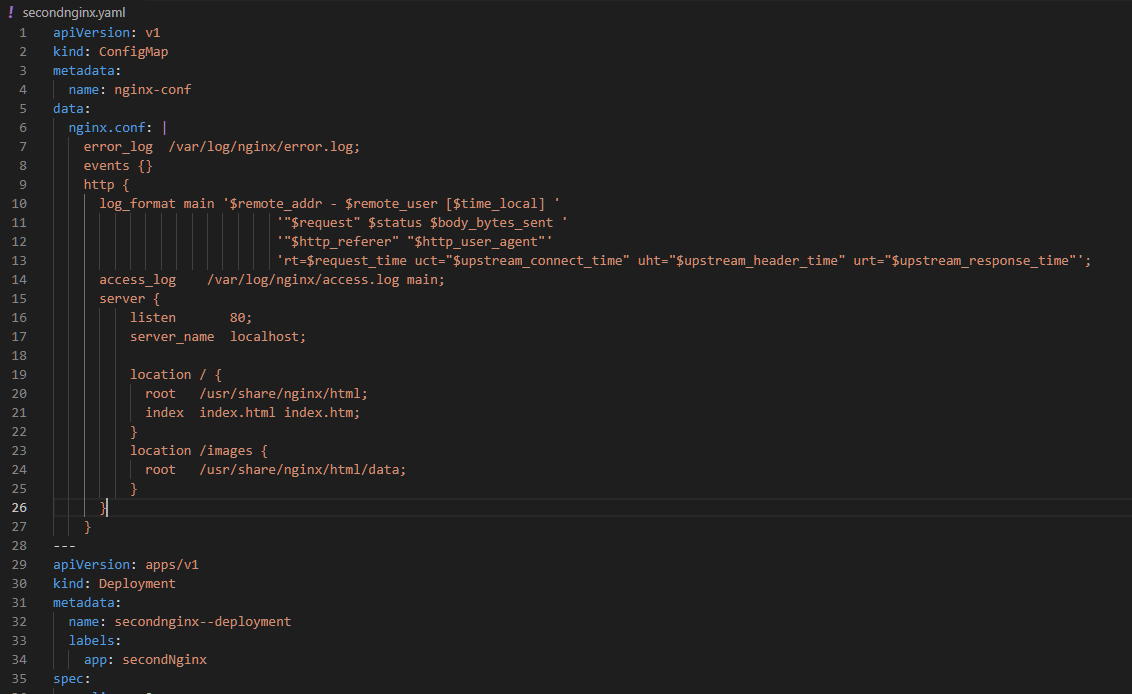
\includegraphics[width=0.95\columnwidth]{images/captures/podnginx/second01.PNG}
	\caption{Archivo de despliegue de deployment .YAML (parte\#1).}
	\label{fig:yml01}
\end{figure}

\begin{figure}[htpb!]
	\centering
	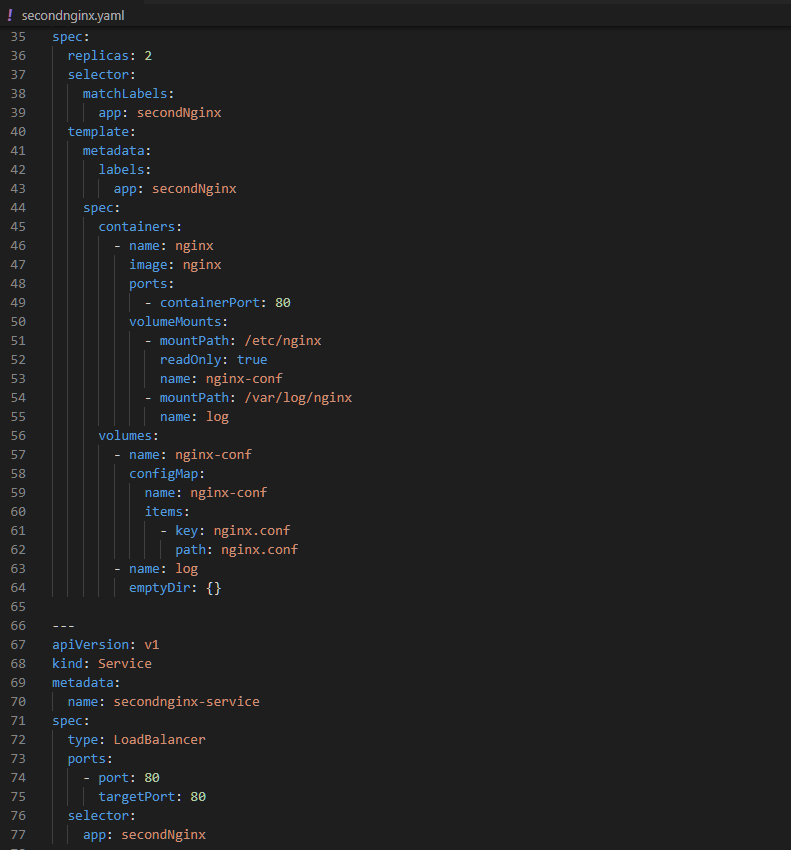
\includegraphics[width=0.95\columnwidth]{images/captures/podnginx/second02.PNG}
	\caption{Archivo de despliegue de deployment .YAML (parte\#2)}
	\label{fig:yml02}
\end{figure}

\par En las figuras \ref{fig:yml01} y \ref{fig:yml02}, se puede observar el archivo .YAML desarrollado para el despliegue de los deployments de Nginx. En dicho el archivo se puede observar características previamente mencionadas, como la creación de 2 replicas de la imagen de Nginx, también se puede ver la creación del servicio y que cada una de estas replicas posee volúmenes del tipo configMap (el cual no es compartido por ambas replicas). En este archivo se configura el uso de los logs de nginx, realizando el cambio necesario dentro del archivo nginx.conf que se encuentra en el volumen de cada pod. Se habilitan los 2 logs, el \textit{error.log} y el \textit{access.log}, el mas relevante sera el log access, ya que se revisara para obtener los tiempos de respuesta por cada solicitud que realiza un cliente al servicio de los deployment. Se le da formato a \textit{access.log} solicitando las variables requeridas para obtener la métrica deseada (el \textit{request time} o tiempo de solicitud, tiempos de respuesta o response time). Es necesario realizar el comando \textbf{kubectl apply -f <deployFile.YAML>} para que se apliquen los cambios y se desplieguen los deployments necesarios con sus respectivos pods y servicios.\\

\par El deployment de Nginx se encarga de servir una pagina simple, en la cual un usuario puede escribir un URL de una imagen para que la pagina la muestre. El documento HTML para el deployment de pruebas cuenta con un peso total de 17628379 bytes (17MB aproximadamente), ambos pods del deployment se encargan de mostrar el mismo sitio por el servicio asignado.\\

\begin{figure}[htpb!]
	\centering
	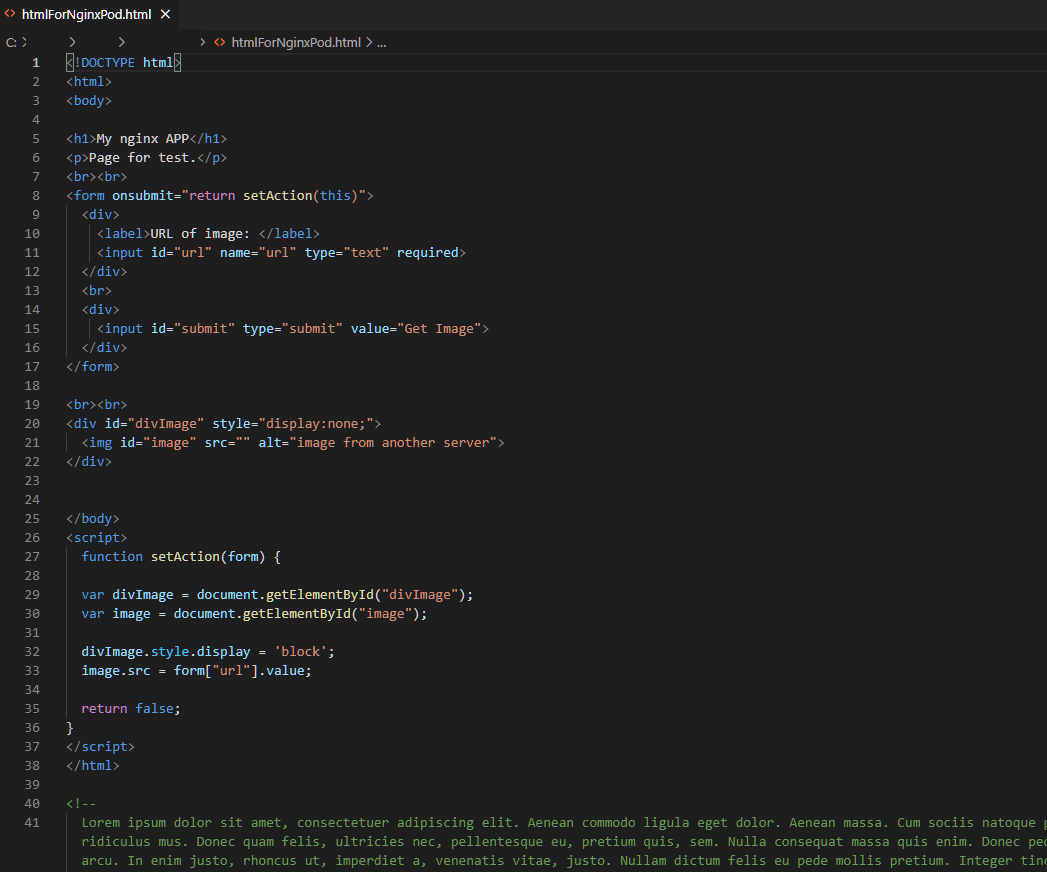
\includegraphics[width=0.95\columnwidth]{images/captures/podnginx/html01.PNG}
	\caption{Archivo Html par los deployments de Nginx.}
	\label{fig:html01}
\end{figure}

\par Se realizo la inserción de una gran cantidad de comentarios (ver Figura \ref{fig:html01}), para incrementar el peso en almacenamiento de la pagina y obtener valores significativos de tiempos de repuesta medibles, es decir, tiempo de respuesta $\textbf{rt > 0.000}$ cuando un cliente realice una solicitud. Para cambiar el index.html de cada pod se uso el comando \textbf{kubectl cp <htmlFileDrirectory>/<htmlFile> <podIdentifier>:/usr/share/nginx/html/index.html} que copia el archivo del equipo al pod. Una vez copiado se puede acceder a la p\'agina, a través de un navegador en un equipo que se encuentre en la red local, para obtener el URL del servicio se ejecuta el comando \textbf{minikube service <serviceName>}, que en este caso es secondnginx-service debido que este es el que se muestra como ejemplo en el .YAML.\\

\par Cada vez que alguien realiza una petición al servicio, dicha solicitud se ve reflejada en el access log de Nginx, el cual puede ser revisado copiando el archivo desde el pod al equipo realizando \textbf{kubectl cp <podIdentifier>:/var/log/nginx/access.log <directoryForCopy>/access.log}, luego se accede al log con uso de un editor de texto como vim o nano y se pueden observar las metricas de request\_time y response\_time.\\ 

\par Así fue implementado en su totalidad el ambiente a usar para probar el funcionamiento de los test, así como, los pods para los experimentos y poder medir métricas simples, de fácil lectura. 
%\subsubsection{Depliegue de pods: Prometheus}
%%%%%%%%%%

\section{Experimentos de inyección de fallas y Resultados}

\par Una vez desarrollado el sistema de inyección de fallas, se realizaron varios experimentos para comprobar su buen funcionamiento y para estudiar el comportamiento de Kubernetes al sufrir fallas. En esta sección se explican los experimentos realizados y se ilustran los resultados obtenidos.\\


\par Para medir objetivamente el desempeño del sistema se debe definir un conjunto de indicadores que nos permitan comparar los resultados obtenidos utilizando distintos casos de prueba.\\


\par Como el funcionamiento del sistema de inyección de fallas depende de cuatro módulos: latencia, CPU, memoria y disco se utilizaran distintos indicadores para cada modulo los cuales se explican a continuación:
\begin{itemize}
    \item Latencia: Se utilizara el ping para su medición, se expresa en milisegundos (ms) es el tiempo que tardan en comunicarse dos puntos en la red.
    \item Memoria RAM: Se expresara su uso en mebibyte (Mi), su equivalencia en bytes es la siguiente: \[ 1\ mebibyte = 1\ Mi = 2^{20}\ bytes = 1.048.576\ bytes \]
    \item CPU: Se utilizara la unidad de Kubernetes llamada millicpu (m) en el cual se divide un núcleo de CPU en 1000 unidades.
    \item Disco: Se expresara con el porcentaje de operaciones de entrada y salida en disco.
    \item Desempeño del pod: Se medira con el tiempo total empleado por Nginx para procesar una solicitud, se expresa en segundos.
\end{itemize} 

\par Esta sección se dividirá en dos partes, la primera en la que se estudiara el correcto funcionamiento de las inyecciones de fallas y la segunda parte en la que se observara y analizará el comportamiento de Kubernetes al sufrir fallas en sus pods.\\

\subsection{Experimentos del funcionamiento de la inyección de fallas}
\carlos{todas las tablas de los resultados no tienen sentido, deben mostrar el estado del cluster en funcion del tiempo}
\carlos{RESPONDER PARA CADA PRUEBA:}

\carlos{- Objetivo}
\carlos{- Por que es interesante medir ese aspecto del desempeño del cluster, por ejemplo, por que es interesante medir la latencia}


\carlos{- Cual es la duracion de cada prueba? Donde se configura? Como se ejecuta?}


\par El grupo de experimentos a continuación demostraran que las pruebas de inyección de fallas están comportándose de la manera esperada.\\ 

\par Cabe destacar que todos los experimentos de esta sección se realizaran en una maquina virtual que utiliza un disco HDD, con dos cores de CPU y 4GB de RAM.\\

\par Se cuantifico un estado estable inicial, sobre los pods de un despliegue de control antes de realizar cualquier test, el cual proporciono las siguientes métricas iniciales, sobre ambos pods del deployment:
\begin{table}[ht!]
\begin{center}
\begin{tabular}{ |c|c| } 
 \hline
 \multicolumn{2}{|c|}{Estado inicial} \\
 \hline
 \hline
 Métrica & Valor(Aprox.)\\
 \hline
 CPU(millicpu) & 0 mCpu\\
 Memoria(mebibytes) & 3 Mi \\
 Request Time (rt) & 0.492 s\\
 \hline
\end{tabular}
\end{center}
\caption{Métricas iniciales Deployment.}
\label{tab:tabla40}
\end{table}

\par Los valores de CPU y Memoria se obtienen utilizando la herramienta del metrics-server de Minikube, siendo consultado varias veces antes de los experimentos. Para medir el Request Time o tiempo de solicitud, se accedió al servicio a través de un navegador sin almacenar cache, luego se realizaron dos solicitudes al servicio por minuto, durante 30 minutos, se reviso el access.log de ambos pod del deployment y se calculo el promedio de los tiempos de solicitud en dicho log.

\subsubsection{Probando el estrés por CPU}

\carlos{Aqui hace falta una grafica que muestre el uso del CPU en funcion del tiempo, en un estado normal}
\carlos{Aqui hace falta una grafica que muestra el uso del CPU en funcion del tiempo mientras se ejecuta el fault injection}

\par Se probara la inyección de falla estudiando el uso inicial del CPU en millicpu (antes del estrés) de un pod de Nginx que tiene dos cores de CPU, luego se estresara al agregarle la sobrecarga de CPU y por ultimo se observara el estado (mientras sucede la falla) para compararlo con el inicial y así demostrar que esta funcionando dicha falla.\\

\par Para obtener el indicador en millicpu en cada estado, se utilizara el comando \\ \verb|kubctl top pods| desde la maquina virtual que tiene alojado a Kubernetes, dicho comando básicamente permite ver el consumo de recursos de los pods.\\

\begin{table}[ht!]
\begin{center}
\begin{tabular}{ |c|c| } 
 \hline
 \multicolumn{2}{|c|}{Resultado} \\
 \hline
 \hline
 Estado & CPU(millicpu)\\
 \hline
 Inicial & 0\\
 Falla & 1658\\
 \hline
\end{tabular}
\end{center}
\caption{Tabla comparativa del uso del CPU en los estados del experimento de estrés por CPU.}
\label{tab:tabla41}
\end{table}


\par Con el resultado se puede observar el aumento sustancial del uso del CPU, el pod afectado durante el estrés esta usando aproximadamente el 80\% del CPU, por lo cual esta funcionando correctamente la inyección de fallas.\\

\subsubsection{Probando el estrés por latencia}

\carlos{Aqui hace falta una grafica que muestre la latencia en funcion del tiempo, en un estado normal}
\carlos{Aqui hace falta una grafica que muestra la latencia en funcion del tiempo mientras se ejecuta el fault injection}

\par Se probara la inyección de falla por latencia estudiando el ping inicial (antes del estrés) de un pod de Nginx, luego se estresara al agregarle un ping de 500ms y por ultimo se observara el estado (mientras sucede la falla) para compararlo con el inicial y así demostrar que esta funcionando dicha falla.\\

\par Para obtener el indicador del ping en cada estado, se utilizara el comando \\ \verb|ping -c 4 <IP del pod afectado>| desde la maquina virtual que tiene alojado a Kubernetes, dicho comando básicamente enviara cuatro solicitudes de ICMP hacia la IP del pod afectado y luego mostrara las respuesta de cada solicitud en la cual se podrá observar el tiempo que tarda cada paquete en llegar a su destino y regresar (ping en ms).\\
\begin{table}[ht!]
\begin{center}
\begin{tabular}{ |c|c| } 
 \hline
 \multicolumn{2}{|c|}{Resultado} \\
 \hline
 \hline
 Estado & Ping(promedio)\\
 \hline
 Inicial & 0.055ms\\
 Falla & 500.5ms\\
 \hline
\end{tabular}
\end{center}
\caption{Tabla comparativa del ping en los estados del experimento de estrés por latencia.}
\label{tab:tabla42}
\end{table}

\vspace{\baselineskip}
\par Con el resultado se puede observar el aumento de 500ms en el ping en el estado de falla, por lo cual esta funcionando correctamente el estrés por latencia.\\

\subsubsection{Probando el estrés por memoria RAM}

\carlos{Aqui hace falta una grafica que muestre el uso de la memoria principal en funcion del tiempo, en un estado normal}
\carlos{Aqui hace falta una grafica que muestra el uso de la ram en funcion del tiempo mientras se ejecuta el fault injection}

\par Se probara la inyección de falla estudiando el uso inicial de memoria RAM en mebibyte (antes del estrés) de un pod de Nginx, luego se estresara al agregarle la sobrecarga de memoria RAM y por ultimo se observara el estado (mientras sucede la falla) para compararlo con el inicial y así demostrar que esta funcionando dicha falla.\\

\par Para obtener el indicador en mebibyte en cada estado, se utilizara el comando \\ \verb|kubctl top pods| desde la maquina virtual que tiene alojado a Kubernetes, dicho comando básicamente permite ver el consumo de recursos de los pods.\\
\begin{table}[ht!]
\begin{center}
\begin{tabular}{ |c|c| } 
 \hline
 \multicolumn{2}{|c|}{Resultado} \\
 \hline
 \hline
 Estado & Memoria(mebibytes)\\
 \hline
 Inicial & 2\\
 Falla & 2059\\
 \hline
\end{tabular}
\end{center}
\caption{Tabla comparativa del porcentaje de uso de la memoria RAM en los estados del experimento de estrés por memoria.}
\label{tab:tabla43}
\end{table}

\vspace{\baselineskip}
\par Con el resultado se puede observar el aumento sustancial del uso de la memoria RAM, por lo cual esta funcionando correctamente la inyección de fallas.\\

\subsubsection{Probando el estrés por disco}

\carlos{Aqui hace falta una grafica que muestre el uso del disco  funcion del tiempo, en un estado normal}
\carlos{Aqui hace falta una grafica que muestra el uso del disco en funcion del tiempo mientras se ejecuta el fault injection}

\par Se probara la inyección de falla estudiando el porcentaje de escritura y lectura inicial del disco (antes del estrés) de un pod de Nginx, luego se estresara al agregarle muchas operaciones al disco y por ultimo se observara el estado (mientras sucede la falla) para compararlo con el inicial y así demostrar que esta funcionando dicha falla.\\

\par Para obtener el indicador en porcentaje en cada estado, se utilizara el comando \\ \verb+iostat -dxy 2 1 | awk '/sda/{print $NF}'+ desde el pod que se utilizara para la prueba, dicho comando básicamente nos mostrara el porcentaje de escritura y lectura del disco sda.\\

%-dxy es estadisticas ampliadas (-x) por dispositivos (-d) omitiendo el primer reporte desde el arranque del sistema (y), 2 seg de espera 1 repeticion y mandamos a imprimir la ultima columna de la fila de sda.  

\begin{table}[ht!]
\begin{center}
\begin{tabular}{ |c|c| } 
 \hline
 \multicolumn{2}{|c|}{Resultado} \\
 \hline
 \hline
 Estado & E/S Disco(porcentaje)\\
 \hline
 Inicial & 1.00\\
 Falla & 96.80\\
 \hline
\end{tabular}
\end{center}
\caption{Tabla comparativa del porcentaje de E/S del disco en los estados del experimento de estrés por disco.}
\label{tab:tabla44}
\end{table}

\par Con el resultado se puede observar el aumento sustancial de las operaciones de escritura y lectura en el disco, por lo cual esta funcionando correctamente la inyección de fallas.\\

\subsection{Experimentos del comportamiento de Kubernetes}

\carlos{Cada experimento debe llevar una grafica en funcion del tiempo (duracion del experimento) donde se pueda apreciar el comportamiento habitual y el fallo que estan inyectando}.

\carlos{que criterio estan utilizando para generar ese "trafico", sobrecarga, o latencia?}

\par En el grupo de experimentos a continuación se busca estudiar el comportamiento de Kubernetes ante fallas.\\ 

\par Se preparo un pod de Nginx que servirá un documento HTML que ocupa 16.8 MB de espacio en disco, a su vez Nginx esta configurado para almacenar los logs de acceso en el cual tendremos la métrica de tiempo de solicitud, dicha variable se estará utilizando para representar el tiempo en segundos que tardo procesar la solicitud y así estudiar el rendimiento durante una falla.\\

\par Se creo un servicio de Kubernetes que servirá dos replicas del pod anteriormente descrito con el fin de comprobar si Kubernetes pudo realizar correctamente el balanceo de carga.\\

\par Cabe destacar que todos los experimentos de esta sección se realizaran en una maquina virtual que utiliza un disco HDD, con dos cores de CPU y 4GB de RAM.\\

\subsubsection{Experimento \#1: Falla de CPU en una replica}

\par Se inyecto la falla de CPU en una replica durante 5 minutos, a continuación el resultado en el rendimiento del servicio.\\
\carlos{como han medido el rendimiento? en funcion del tiempo de respuesta de la aplicacion? que aplicacion está funcionando?}
\begin{table}[ht!]
\begin{center}
\begin{tabular}{ |c|c| } 
 \hline
 \multicolumn{2}{|c|}{Resultado} \\
 \hline
 \hline
 Estado & Tiempo de solicitud(segundos)\\
 \hline
 Inicial & 0.492\\
 Falla & 1.300\\
 \hline
\end{tabular}
\end{center}
\caption{Tabla comparativa del tiempo de solicitud en los estados del experimento \#1.}
\label{tab:tabla45}
\end{table}


\par Se pudo observar que el pod afectado utilizo entre 1500 y 1700 de mCPU durante la falla. También se observ\'o que, Kubernetes logro hacer un balanceo de carga ya que la replica que respondió las solicitudes no fue la que se encontraba afectada con la falla del CPU, sin embargo, se pudo notar un leve aumento en el tiempo de solicitud porque el CPU del nodo en general se vio comprometido con la falla.\\

\subsubsection{Experimento \#2: Falla de CPU en dos replicas}

\par Se inyecto la falla de CPU en las dos replicas durante 15 minutos, a continuación el resultado en el rendimiento del servicio.\\

\begin{table}[ht!]
\begin{center}
\begin{tabular}{ |c|c| } 
 \hline
 \multicolumn{2}{|c|}{Resultado} \\
 \hline
 \hline
 Estado & Tiempo de solicitud(segundos)\\
 \hline
 Inicial & 0.492\\
 Falla & 10.037\\
 \hline
\end{tabular}
\end{center}
\caption{Tabla comparativa del tiempo de solicitud en los estados del experimento \#2.}
\label{tab:tabla46}
\end{table}

\par Se pudo observar un aumento considerable del tiempo de solicitud, Kubernetes repartió el total del CPU disponible entre las 2 replicas, cada una con un uso entre 800 y 900 de mCPU (entre 1600 y 1700 total entre ambas) sin embargo esto no resuelve la falla simplemente realizo un balanceo del recurso en el nodo.\\

\subsubsection{Experimento \#3: Falla de disco en una replica}

\par Se inyecto la falla de disco en una replica durante 5 minutos, a continuación el resultado en el rendimiento del servicio.\\

\begin{table}[ht!]
\begin{center}
\begin{tabular}{ |c|c| } 
 \hline
 \multicolumn{2}{|c|}{Resultado} \\
 \hline
 \hline
 Estado & Tiempo de solicitud(segundos)\\
 \hline
 Inicial & 0.492\\
 Falla & 1.900\\
 \hline
\end{tabular}
\end{center}
\caption{Tabla comparativa del tiempo de solicitud en los estados del experimento \#3.}
\label{tab:tabla47}
\end{table}

\par Se pudo notar que Kubernetes respondió las solicitudes con ambas replicas (la que poseía la falla y la que no, es decir, no hubo balanceo en esta falla), en ambas replicas se pudo notar un leve aumento en el tiempo de solicitud ya que ambas replicas comparten el mismo disco del nodo, aunque cada una posee su propio volumen y solo era afectado el uso de disco en el pod con falla.\\

\subsubsection{Experimento \#4: Falla de disco en dos replicas}

\par Se inyecto la falla de disco en las dos replicas durante 15 minutos, a continuación el resultado en el rendimiento del servicio.\\

\begin{table}[ht!]
\begin{center}
\begin{tabular}{ |c|c| } 
 \hline
 \multicolumn{2}{|c|}{Resultado} \\
 \hline
 \hline
 Estado & Tiempo de solicitud(segundos)\\
 \hline
 Inicial & 0.492\\
 Falla & 3.700\\
 \hline
\end{tabular}
\end{center}
\caption{Tabla comparativa del tiempo de solicitud en los estados del experimento \#4.}
\label{tab:tabla48}
\end{table}

\par Se pudo observar un leve aumento (a diferencia de las otras pruebas sobre ambos pods) del tiempo de solicitud, ambas replicas dieron respuesta a las solicitudes, Kubernetes no se pudo recuperar de esta falla durante el tiempo que duro el experimento.\\

\subsubsection{Experimento \#5: Falla por latencia en una replica}

\par Se inyecto la falla por latencia en una replica durante 5 minutos, a continuación el resultado en el rendimiento del servicio.\\

\begin{table}[ht!]
\begin{center}
\begin{tabular}{ |c|c| } 
 \hline
 \multicolumn{2}{|c|}{Resultado} \\
 \hline
 \hline
 Estado & Tiempo de solicitud(segundos)\\
 \hline
 Inicial & 0.492\\
 Falla & 0.820\\
 \hline
\end{tabular}
\end{center}
\caption{Tabla comparativa del tiempo de solicitud en los estados del experimento \#5.}
\label{tab:tabla49}
\end{table}

\par Se pudo observar que Kubernetes logro hacer un balanceo de carga ya que la replica que respondió las solicitudes no fue la que se encontraba con latencia inyectada, dicha replica sin fallas no se vio afectada por el estrés que se le realizo a su replica hermana, no hubo incremento en el tiempo de respuesta del servicio debido al balanceo.\\

\subsubsection{Experimento \#6: Falla por latencia en las dos replicas}

\par Se inyecto la falla por latencia en dos replicas durante 15 minutos, a continuación el resultado en el rendimiento del servicio.\\

\begin{table}[ht!]
\begin{center}
\begin{tabular}{ |c|c| } 
 \hline
 \multicolumn{2}{|c|}{Resultado} \\
 \hline
 \hline
 Estado & Tiempo de solicitud(segundos)\\
 \hline
 Inicial & 0.492\\
 Falla & 6.820\\
 \hline
\end{tabular}
\end{center}
\caption{Tabla comparativa del tiempo de solicitud en los estados del experimento \#6.}
\label{tab:tabla50}
\end{table}

\par Se pudo observar un aumento considerable del tiempo de solicitud, ambas replicas se encontraban afectadas con 500ms de latencia, Kubernetes no se pudo recuperar de esta falla durante el tiempo que duro el experimento.\\

\subsubsection{Experimento \#7: Falla de memoria RAM en una replica}

\par Se inyecto la falla de memoria RAM en una replica durante 5 minutos, a continuación el resultado en el rendimiento del servicio.\\

\begin{table}[ht!]
\begin{center}
\begin{tabular}{ |c|c| } 
 \hline
 \multicolumn{2}{|c|}{Resultado} \\
 \hline
 \hline
 Estado & Tiempo de solicitud(segundos)\\
 \hline
 Inicial & 0.492\\
 Falla & 1.592\\
 \hline
\end{tabular}
\end{center}
\caption{Tabla comparativa del tiempo de solicitud en los estados del experimento \#7.}
\label{tab:tabla51}
\end{table}

\par Se pudo observar al pod afectado con un mayo de 2100 MiB de memoria. También que Kubernetes logro hacer un balanceo de carga ya que la replica que respondió las solicitudes no fue la que se encontraba con la falla, sin embargo, se pudo notar un leve aumento en el tiempo de solicitud del servicio, porque la memoria del nodo en general se vio comprometido con la falla.//

\subsubsection{Experimento \#8: Falla de memoria RAM en dos replicas}

\par Se inyecto la falla de memoria RAM en las dos replicas durante 15 minutos, a continuación el resultado en el rendimiento del servicio.\\

\begin{table}[ht!]
\begin{center}
\begin{tabular}{ |c|c| } 
 \hline
 \multicolumn{2}{|c|}{Resultado} \\
 \hline
 \hline
 Estado & Tiempo de solicitud(segundos)\\
 \hline
 Inicial & 0.492\\
 Falla & 4.164\\
 \hline
\end{tabular}
\end{center}
\caption{Tabla comparativa del tiempo de solicitud en los estados del experimento \#8.}
\label{tab:tabla52}
\end{table}

\par Se pudo observar un aumento considerable del tiempo de solicitud, ambas replicas poseían entre 1700 y 2000 MiB de memoria en uso cada una, no los 2048 mínimos de la falla (el total de uso entre ambos no supero los 4096 MiB total del nodo), Kubernetes no se pudo recuperar de esta falla durante el tiempo que duro el experimento y se observo notificaciones de procesos encargados de inyectar fallas detro de los pods, siendo eliminados por el sistema operativo del nodo, debido al evento OOM (\textit{Out of Memory}).\\
